% ==========================================================================
%  DRAFT for IEEE Internet of Things Journal  (IEEEtran journal format)
%  SUBMISSION TYPE: TRADITIONAL (NOT open access)  ->  US$ 0 publication fee
%  HARD LIMIT: 8 published pages incl. references + biographies.
%  Every page above 8 costs US$ 175 (mandatory). Run  check_pages.bat
%  Everything marked \TODO{} needs REAL field data or author input.
%  Do NOT fill result tables with simulator output.
%
%  Page budget (8 pages total):
%    Title+Abstract+Intro ............ 1.0   Sec. II Machine & model .... 1.0
%    Sec. III Architecture ........... 1.25  Sec. IV Setup .............. 0.75
%    Sec. V Results (4 subsections) .. 2.25  Sec. VI Discussion+Concl ... 0.5
%    References (~30) + bios ......... 1.25
% ==========================================================================
\documentclass[journal]{IEEEtran}
\usepackage{amsmath,amssymb,graphicx,booktabs,xcolor,tikz,cite,url}
\usetikzlibrary{positioning,arrows.meta,fit}
\newcommand{\TODO}[1]{\textcolor{red}{[TODO: #1]}}

\begin{document}
\title{An IoT-Enabled Hybrid Soft Sensor for Real-Time Residual-Moisture Monitoring and Resource Accounting in Compact Wool Scouring Machines}

\author{Robiya~Tuguzbaeva,
        Sherkul~Khakimov,
        Firuza~Dustova,
        and~Ruzimurod~Rosulov%
\thanks{The authors are with the Tashkent Institute of Textile and
Light Industry, 5 Shohjahon Street, Tashkent 100100, Uzbekistan (e-mail: trobiya89@mail.ru;
lionandlion9@mail.ru; firuzadustovahamraevna@mail.ru; rasulov.ruzimurad@mail.ru).}%
\thanks{ORCID iDs: R.~Tuguzbaeva 0009-0001-8480-9696;
S.~Khakimov 0000-0002-1933-1948;
F.~Dustova 0009-0007-5928-3198;
R.~Rosulov 0000-0003-0590-3121.}%
\thanks{Corresponding author: Robiya Tuguzbaeva (e-mail: trobiya89@mail.ru).}%
\thanks{\TODO{Funding: state grant 7/275, etc.}}}

% Running head shown on pages 2+ (IEEE style)
\markboth{IEEE Internet of Things Journal}%
{Tuguzbaeva \MakeLowercase{\textit{et al.}}: IoT-Enabled Hybrid Soft Sensor for Wool Scouring Machines}

\maketitle

\begin{abstract}
Wool scouring is among the most water- and energy-intensive steps in primary wool processing, yet small regional
plants operate their machines without any instrumentation, and the key quality variable---residual moisture of the wool
after each squeeze stage---is measured only occasionally by oven drying. This paper presents a low-cost Internet of Things
(IoT) framework for a compact five-bowl wool scouring machine with an improved ribbed-drum/mesh squeezing device.
An ESP32-based edge node acquires bowl temperature, liquor level and turbidity, squeeze-drum angular speed, make-up
water flow and electrical power, and streams them over Wi-Fi (HTTP/MQTT) to a server that provides storage, alarms,
per-kilogram resource indicators and a bilingual web/mobile application. We propose a hybrid soft sensor in which a
design-of-experiments (DoE) regression model of the squeezing device, obtained from a $2^3$ full-factorial experiment,
serves as a physics-informed prior, and an online ridge-regression correction learned from sparse laboratory samples
accounts for operating conditions. In a \TODO{N}-shift field deployment at \TODO{plant}, the soft sensor achieved an RMSE
of \TODO{x}\,\% against oven-dry reference measurements, compared with \TODO{y}\,\% for the DoE model alone and
\TODO{z}\,\% for a purely data-driven model, while the system delivered \TODO{packet-delivery ratio}\,\% of messages with a
median latency of \TODO{ms}. The measured specific energy and water consumption were \TODO{kWh/kg} and \TODO{L/kg}.
\end{abstract}

\begin{IEEEkeywords}
Industrial Internet of Things, soft sensor, wool scouring, edge computing, resource efficiency, textile manufacturing, digital twin.
\end{IEEEkeywords}

% --------------------------------------------------------------------------
\section{Introduction}
\IEEEPARstart{P}{rimary} wool processing---opening, scouring, squeezing and drying---determines the quality and cost of
all downstream textile products. Scouring removes grease, suint and mineral dirt in a sequence of bowls filled with hot
alkaline liquor; between bowls, squeezing devices remove the dirty liquor from the wool. Insufficient squeezing carries
dirt into the next bowl, shortens liquor life and increases water and detergent consumption, and every percentage point
of residual moisture must later be evaporated in the dryer.

In regions such as Uzbekistan, where wool comes largely from Karakul sheep and is processed in small, decentralised
plants, large centralised scouring lines are uneconomic. A compact, resource-saving machine with an improved squeezing
device (ribbed squeeze drum, guide slat drum and wrapped mesh surface) was developed and patented in previous work
\cite{tuguzbayeva2024,patent02351}; factory tests reported a reduction of residual moisture from 65--70\,\% to
55--60\,\% and of installed power from 13 to 4.2\,kW. However, such machines are operated without sensors: operators
cannot see liquor temperature or dirtiness, moisture is measured only by occasional oven-dry samples, and resource
consumption is not accounted per kilogram of wool.

Industrial IoT \cite{xu2014iot} and soft sensing \cite{kadlec2009soft} offer a remedy, but published IoT work in textiles
focuses on spinning, weaving and dyeing; \TODO{add 6--10 recent IoT/textile/soft-sensor references, 2020--2025, incl.
IEEE IoT-J papers} --- to our knowledge, no work instruments the scouring/squeezing stage or exploits DoE models of the
machine as a prior for an IoT soft sensor.

\textbf{Contributions.}
\begin{enumerate}
\item A low-cost ($\approx$\,US\$\,200) IoT architecture for wool scouring machines with an ESP32 edge node, HTTP/MQTT
transport, server-side analytics and an installable bilingual (EN/RU) web/mobile application.
\item A hybrid soft sensor for residual moisture that combines a $2^3$ factorial regression model of the squeezing device
(geometry prior) with an online, regularised correction for operating conditions, calibrated from sparse laboratory samples.
\item Real-time per-kilogram resource indicators (kWh/kg, L/kg) and rule-based fault alarms (heater failure, low level,
dirty liquor, drum speed deviation).
\item A field deployment on an industrial machine with \TODO{N} shifts of data, an open dataset and code \TODO{repo URL}.
\end{enumerate}

% --------------------------------------------------------------------------
\section{Machine and Squeezing Model}
The machine comprises five bowls (2.5\,m$^3$ each); moving rakes (length 250\,mm, linear speed \TODO{0.15}\,m/s) transport
the wool, and each bowl is followed by a squeezing device with a ribbed drum of diameter $D$, a mesh of hole diameter
$d$ and a drum--mesh gap $h$ \cite{tuguzbayeva2024}.

\subsection{DoE prior}
A $2^3$ full-factorial experiment with three replicates ($N=8$, $m=3$) with coded factors
$X_1=(d-2)/1$, $X_2=(D-250)/50$, $X_3=(h-3)/1$ (mm) gave, after Student's test ($t_{0.05;16}=2.12$), the adequate model
($F=0.71<F_{0.05;4;16}=3.01$)
\begin{equation}
W_0 = 57.31 + 0.81X_1 - 0.95X_2 + 0.30X_3 \quad [\%].
\label{eq:prior}
\end{equation}

\subsection{Hybrid soft sensor}
Equation~\eqref{eq:prior} captures geometry only. During operation, moisture also depends on the drum angular speed
$\omega$, the feed rate $q$, the liquor temperature $T$ and the liquor turbidity $\tau$. With normalised deviations
$\boldsymbol\phi=[(\omega-\omega_0)/s_\omega,\,(q-q_0)/s_q,\,(T-T_0)/s_T,\,(\tau-\tau_0)/s_\tau]^\top$ we model
\begin{equation}
\hat W = W_0(d,D,h) + \mathbf w^\top\boldsymbol\phi + c,
\end{equation}
where $(\mathbf w,c)$ minimise $\sum_i (W_i - W_{0,i} - \mathbf w^\top\boldsymbol\phi_i - c)^2 + \lambda\|\mathbf w\|^2$
over laboratory samples $W_i$ taken after the squeezer and dried at 105\,$^\circ$C. The model is refitted on the server
each time a sample is added; with no samples it reduces to the DoE prior.
\TODO{Compare with: DoE only; ridge/GPR/random forest without prior; report learning curve vs number of samples.}

% --------------------------------------------------------------------------
\section{IoT System Architecture}
\begin{figure}[t]
\centering
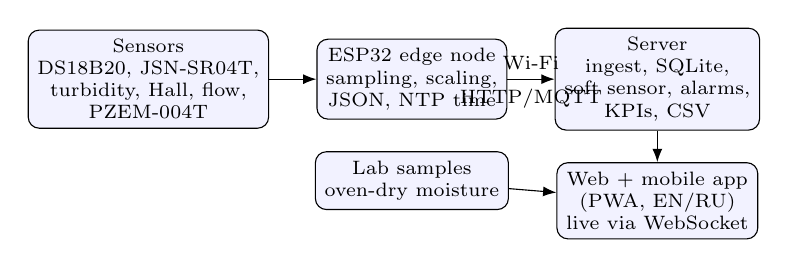
\begin{tikzpicture}[font=\scriptsize, node distance=4mm and 6mm,
  b/.style={draw,rounded corners,align=center,minimum height=7mm,fill=blue!5}]
\node[b] (s) {Sensors\\DS18B20, JSN-SR04T,\\turbidity, Hall, flow,\\PZEM-004T};
\node[b,right=of s] (e) {ESP32 edge node\\sampling, scaling,\\JSON, NTP time};
\node[b,right=of e] (srv) {Server\\ingest, SQLite,\\soft sensor, alarms,\\KPIs, CSV};
\node[b,below=of srv] (app) {Web + mobile app\\(PWA, EN/RU)\\live via WebSocket};
\node[b,below=of e] (lab) {Lab samples\\oven-dry moisture};
\draw[-{Latex}] (s)--(e); \draw[-{Latex}] (e)--node[above]{Wi-Fi}node[below]{HTTP/MQTT}(srv);
\draw[-{Latex}] (srv)--(app); \draw[-{Latex}] (lab)--(app);
\end{tikzpicture}
\caption{Architecture of the proposed IoT framework.}
\label{fig:arch}
\end{figure}
Fig.~\ref{fig:arch} shows the architecture. \TODO{Describe sensor placement (photo), sampling period (2\,s), payload
size, power supply, enclosure, calibration of each sensor (method and uncertainty).}

% --------------------------------------------------------------------------
\section{Experimental Setup}
\TODO{Plant, dates, wool type (spring/autumn Karakul), number of shifts, lab sampling protocol (every 30 min, 3 replicates),
train/test split by day, network environment (AP distance, RSSI).}

% --------------------------------------------------------------------------
\section{Results}
\subsection{Soft-sensor accuracy}
\begin{table}[t]\centering\caption{Residual-moisture prediction on held-out field samples}
\begin{tabular}{lccc}\toprule
Model & RMSE (\%) & MAE (\%) & $R^2$\\\midrule
DoE prior only \eqref{eq:prior} & \TODO{} & \TODO{} & \TODO{}\\
Data-driven ridge (no prior) & \TODO{} & \TODO{} & \TODO{}\\
Random forest (no prior) & \TODO{} & \TODO{} & \TODO{}\\
\textbf{Hybrid (proposed)} & \TODO{} & \TODO{} & \TODO{}\\\bottomrule
\end{tabular}\end{table}

\subsection{Resource indicators}
\TODO{kWh/kg and L/kg per shift, baseline vs improved machine, mean $\pm$ SD, $n$.}

\subsection{Communication performance}
\TODO{Packet delivery ratio, latency distribution, outages, energy of node.}

\subsection{Fault detection}
\TODO{Detection delay and false-alarm rate for heater-off, low-level, drum-speed scenarios.}

% --------------------------------------------------------------------------
\section{Discussion and Limitations}
\TODO{Generalisation across wool types, sensor fouling (turbidity probes in alkaline liquor), Wi-Fi in wet halls,
scaling to multiple plants, security (device token, TLS).}

\section{Conclusion}
\TODO{}

\bibliographystyle{IEEEtran}
\begin{thebibliography}{9}
\bibitem{tuguzbayeva2024} R.~B. Tuguzbayeva, ``Improvement of the working parts of a wool washing machine,'' Ph.D.
dissertation, Tashkent Inst. Textile Light Ind., Tashkent, Uzbekistan, 2024.
\bibitem{patent02351} R.~B. Tuguzbayeva \emph{et al.}, ``Device for squeezing wool in a wool washing bowl,'' Uzbekistan
Utility Model Patent FAP~02351, 2023. \TODO{check inventors}
\bibitem{xu2014iot} L.~D. Xu, W.~He, and S.~Li, ``Internet of things in industries: A survey,'' \emph{IEEE Trans. Ind.
Informat.}, vol.~10, no.~4, pp.~2233--2243, Nov. 2014.
\bibitem{kadlec2009soft} P.~Kadlec, B.~Gabrys, and S.~Strandt, ``Data-driven soft sensors in the process industry,''
\emph{Comput. Chem. Eng.}, vol.~33, no.~4, pp.~795--814, 2009.
\bibitem{tao2019dt} F.~Tao, H.~Zhang, A.~Liu, and A.~Y.~C. Nee, ``Digital twin in industry: State-of-the-art,''
\emph{IEEE Trans. Ind. Informat.}, vol.~15, no.~4, pp.~2405--2415, Apr. 2019.
\bibitem{montgomery} D.~C. Montgomery, \emph{Design and Analysis of Experiments}, 9th~ed. Hoboken, NJ, USA: Wiley, 2017.
\end{thebibliography}

% Short biographies WITHOUT photos save ~0.3 page (photos are optional at first submission;
% the editor may ask for them in the final version - keep bios to 3-4 lines each).
\begin{IEEEbiographynophoto}{Robiya Tuguzbaeva}
received the Ph.D. degree in technical sciences from the Tashkent Institute of Textile and Light Industry,
Tashkent, Uzbekistan, in \TODO{year}, and is currently an Assistant Professor with the Department of Natural Fiber
Technology and Engineering, Tashkent Institute of Textile and Light Industry. Research interests include
wool processing machinery, resource-efficient textile technology, and industrial IoT.
\end{IEEEbiographynophoto}
\begin{IEEEbiographynophoto}{Sherkul Khakimov}
is a Professor with the Tashkent Institute of Textile and Light Industry, Tashkent, Uzbekistan. \TODO{2--3 lines.}
\end{IEEEbiographynophoto}
\begin{IEEEbiographynophoto}{Firuza Dustova}
is with the Tashkent Institute of Textile and Light Industry, Tashkent, Uzbekistan. \TODO{2--3 lines.}
\end{IEEEbiographynophoto}
\begin{IEEEbiographynophoto}{Ruzimurod Rosulov}
is with the Tashkent Institute of Textile and Light Industry, Tashkent, Uzbekistan. \TODO{2--3 lines.}
\end{IEEEbiographynophoto}
\end{document}
